\documentclass{article}
\usepackage{tikz-qtree}
\begin{document}
 \tikzset{edge from parent/.style=
     {draw, edge from parent path={(\tikzparentnode) -- (\tikzchildnode)}}}
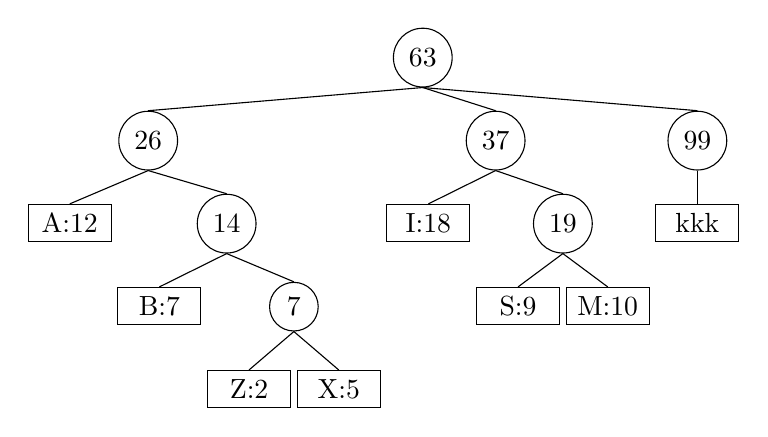
\begin{tikzpicture}[every leaf node/.style={draw,rectangle,minimum width={3em}},
                    every internal node/.style={draw,circle}]
\Tree
 [.63 
    [.26 A:12 
        [.14 B:7 
            [.7 Z:2 X:5 ]
        ]
    ] 
    [.37 I:18 
        [.19 S:9 M:10  ]
    ]
    [.99 kkk ]
]
\end{tikzpicture}

\end{document}
